


\begin{frame}[fragile]{Proposed Method: K-Graph}
  \begin{figure}
    \centering
  \subfloat{ 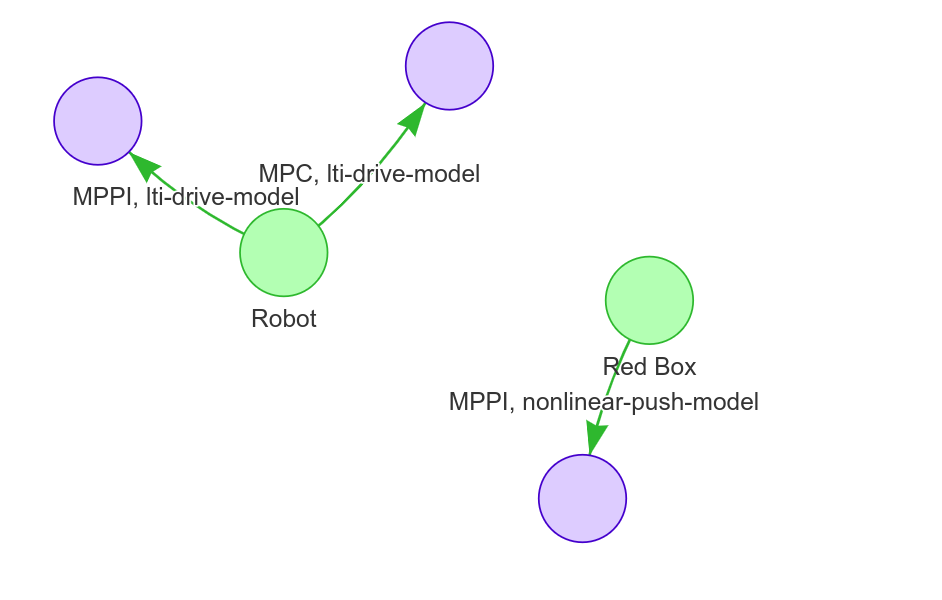
\includegraphics[height=0.8\textheight]{figures/proposed_method/kgraph_testing_phase} }
  \subfloat{ 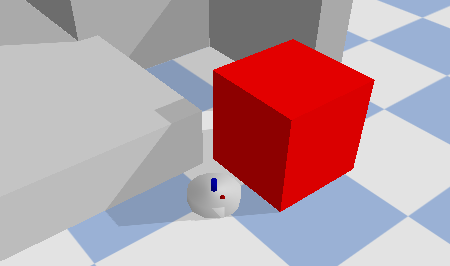
\includegraphics[height=0.3\textheight]{figures/introduction/example_env}}
\end{figure}
\end{frame}


% \begin{frame}[fragile]{Proposed Method: K-Graph}
% Formally, a \textbf{\acl{k-graph}}, $\gls{k-graph} = \left\langle \gls{nodesK}, \gls{edgesK} \right\rangle $
% \\comprising $\gls{nodesK} = \{\gls{node}^{\mathit{center}}, \gls{node}^{\mathit{side}}\}$, \quad $\gls{edgesK} \in \{\gls{edge}_{(i,j)}| i \in \gls{nodesK}^\mathit{center}_\mathit{ids}, j \in \gls{nodesK}^\mathit{side}_\mathit{ids} \}$.\bs
% \end{frame}


\begin{frame}[fragile]{Proposed Method: K-Graph}
  % 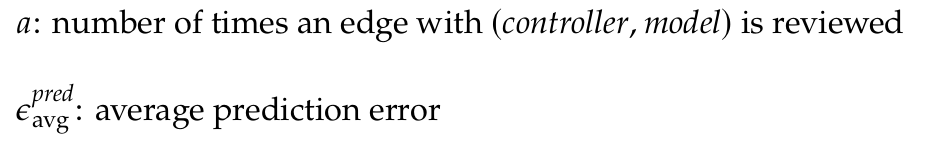
\includegraphics[width=0.8\textwidth]{figures/proposed_method/explain_successf}\pause

  Action Feedback $\alpha$:\bs

  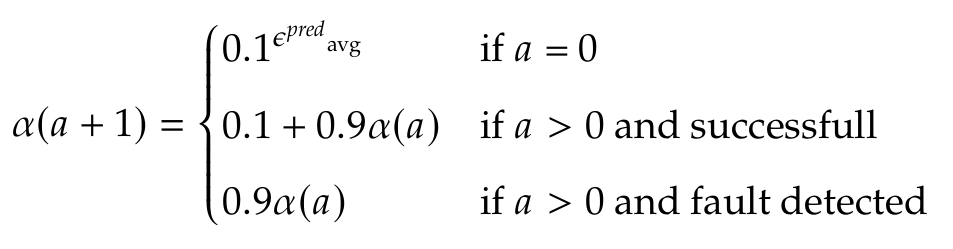
\includegraphics[width=0.7\textwidth]{figures/proposed_method/successfactor}

 $a$: number of times (\textit{controller}, \textit{model}) received action feedback\bs

 ${\epsilon^\mathit{pred}}_{avg}$: average prediction error\bs
\end{frame}
